\documentclass[margin=2pt]{standalone}
\usepackage{circuitikz, amsmath, siunitx,tikz,pgfplots}
\pgfplotsset{compat=1.18}
\usetikzlibrary{arrows}
\usetikzlibrary{decorations.markings}
\pgfsetarrowoptions{direction ee}{5pt}
\usetikzlibrary{circuits.ee.IEC}
\usetikzlibrary {circuits}
\begin{document}

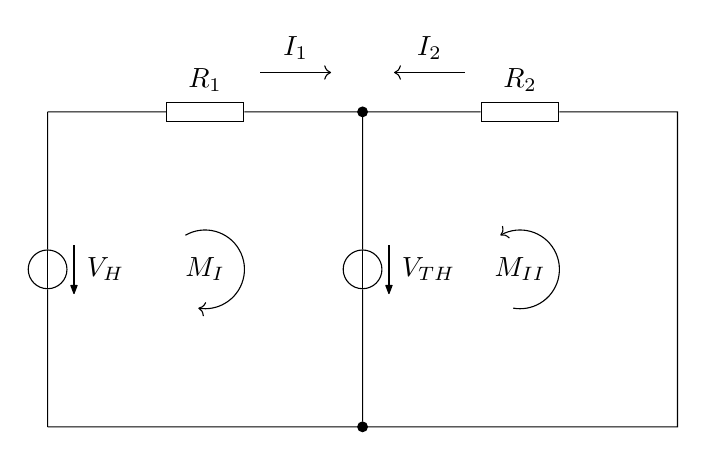
\begin{tikzpicture}[circuit ee IEC]
    \def\ang{120}
    \def\a{0.5}
    \def\b{0.5}
    \node[contact] (top) at (4,4) {};
    \node[contact] (bottom) at (4,0) {};
    \draw
    (0,4) to [voltage source = {direction info = {info = $V_H$}}] (0,0);
    \draw (0,4)  to [R = {info = {$R_1$}}] (4,4)

    to [R = {info = {$R_2$}}] (8,4)
    to [short] (8,0)
    to [short] (0,0)

    (top)   to [voltage source = {direction info= {info = $V_{TH}$}}] (bottom);

    \draw[->] (2.7, 4.5) --++ (0.9,0) node[midway,above=1] {$I_1$};
    \draw[<-] (8-2.7-0.9, 4.5) --++ (0.9,0) node[midway,above=1] {$I_2$};
    \draw[->] ({2+\a*cos(\ang)},{2+\b*sin(\ang)}) arc (120:-100:{\a} and {\b});
    \node[] at (2,2) {$M_I$};
    \draw[<-] ({2+4+ \a*cos(\ang)},{2+\b*sin(\ang)}) arc (120:-100:{\a} and {\b});
    \node[] at (2+4,2) {$M_{II}$};

\end{tikzpicture}
\end{document}